\documentclass[a4paper, 14pt]{extarticle}

% Поля
%--------------------------------------
\usepackage{geometry}
\geometry{a4paper,tmargin=2cm,bmargin=2cm,lmargin=3cm,rmargin=1cm}
%--------------------------------------


%Russian-specific packages
%--------------------------------------
\usepackage[T2A]{fontenc}
\usepackage[utf8]{inputenc}
\usepackage[english, main=russian]{babel}
%--------------------------------------

\usepackage{textcomp}

% Красная строка
%--------------------------------------
\usepackage{indentfirst}
%--------------------------------------


%Graphics
%--------------------------------------
\usepackage{graphicx}
\graphicspath{ {./images/} }
\usepackage{wrapfig}
%--------------------------------------

% Полуторный интервал
%--------------------------------------
\linespread{1.3}
%--------------------------------------

%Выравнивание и переносы
%--------------------------------------
\sloppy
\clubpenalty=10000
\widowpenalty=10000
%--------------------------------------

%Списки
\usepackage{enumitem}

%Подписи
\usepackage{caption}

%Гиперссылки
\usepackage{hyperref}

\hypersetup {
 unicode=true
}

%Рисунки
%--------------------------------------
\DeclareCaptionLabelSeparator*{emdash}{~--- }
\captionsetup[figure]{labelsep=emdash,font=onehalfspacing,position=bottom}
%--------------------------------------

\usepackage{tempora}

\usepackage{listings}
\usepackage{xcolor}

\lstset{
    basicstyle=\ttfamily,
    breaklines=true,
    columns=fullflexible,
    frame=single,
    inputencoding=utf8,
    extendedchars=true,
    keywordstyle=\bf,
    numbers=left,
    numbersep=5pt,
    xleftmargin=25pt,
    xrightmargin=25pt,
}


%--------------------------------------
%   НАЧАЛО ДОКУМЕНТА
%--------------------------------------

\usepackage{array}
\usepackage{tabularx}
\usepackage{float}
\newcolumntype{L}[1]{>{\raggedright\arraybackslash}p{#1}}
\newcolumntype{Y}{>{\raggedright\arraybackslash}X}
\captionsetup[table]{labelsep=emdash,justification=raggedright,singlelinecheck=false,font=small,skip=5pt}

\begin{document}

%--------------------------------------
%   ТИТУЛЬНЫЙ ЛИСТ
%--------------------------------------
\begin{titlepage}
\thispagestyle{empty}
\newpage


%Шапка титульного листа
%--------------------------------------
\vspace*{-60pt}
\hspace{-65pt}
\begin{minipage}{0.3\textwidth}
\hspace*{-20pt}\centering

\includegraphics[width=\textwidth]{emblem}
\end{minipage}
\begin{minipage}{0.67\textwidth}\small \textbf{
\vspace*{-0.7ex}
\hspace*{-6pt}\centerline{Министерство науки и высшего образования Российской Федерации}
\vspace*{-0.7ex}
\centerline{Федеральное государственное бюджетное образовательное учреждение }
\vspace*{-0.7ex}
\centerline{высшего образования}
\vspace*{-0.7ex}
\centerline{<<Московский государственный технический университет}
\vspace*{-0.7ex}
\centerline{имени Н.Э. Баумана}
\vspace*{-0.7ex}
\centerline{(национальный исследовательский университет)>>}
\vspace*{-0.7ex}
\centerline{(МГТУ им. Н.Э. Баумана)}}
\end{minipage}
%--------------------------------------

%Полосы
%--------------------------------------
\vspace{-25pt}
\hspace{-35pt}\rule{\textwidth}{2.3pt}

\vspace*{-20.3pt}
\hspace{-35pt}\rule{\textwidth}{0.4pt}
%--------------------------------------

\vspace{1.5ex}
\hspace{-35pt} \noindent \small ФАКУЛЬТЕТ\hspace{80pt} <<Информатика и системы управления>>

\vspace*{-16pt}
\hspace{47pt}\rule{0.83\textwidth}{0.4pt}

\vspace{0.5ex}
\hspace{-35pt} \noindent \small КАФЕДРА\hspace{50pt} <<Теоретическая информатика и компьютерные технологии>>

\vspace*{-16pt}
\hspace{30pt}\rule{0.866\textwidth}{0.4pt}

\vspace{11em}

\begin{center}
\Large {\bf Лабораторная работа № 3} \\

\large {\bf по курсу <<Базы данных>>} \\[0.8cm]

\large <<Преобразование модели <<сущность--связь>>\\
в реляционную модель>>
\end{center}
\normalsize

\vspace{8em}


\begin{flushright}
  {Студент группы ИУ9-51Б Хромов М.А. \hspace*{15pt}\\
  \vspace{2ex}
  Преподаватель Вишняков И. Э.\hspace*{15pt}}
\end{flushright}

\bigskip

\vfill


\begin{center}
\textsl{Москва 2026}
\end{center}
\end{titlepage}


% =================================================
% ОСНОВНАЯ ЧАСТЬ
% =================================================

\setcounter{page}{2}

\section{Задача}
\begin{enumerate}
  \item Преобразовать модель <<сущность--связь>>, созданную в лабораторной работе № 1, в реляционную модель согласно процедуре преобразования.
  \item Обосновать выбор типов данных, ключей и правил обеспечения ограничений минимальной кардинальности.
\end{enumerate}

\section{Практическая реализация}
\subsection{Построение реляционной модели}
Предметная область <<Турнирный оператор>> включает организаторов, дисциплины, турниры, команды и сведения об их участии. Исходная модель представлена на рисунке~\ref{fig:er-model}.

\begin{figure}[H]
  \centering
  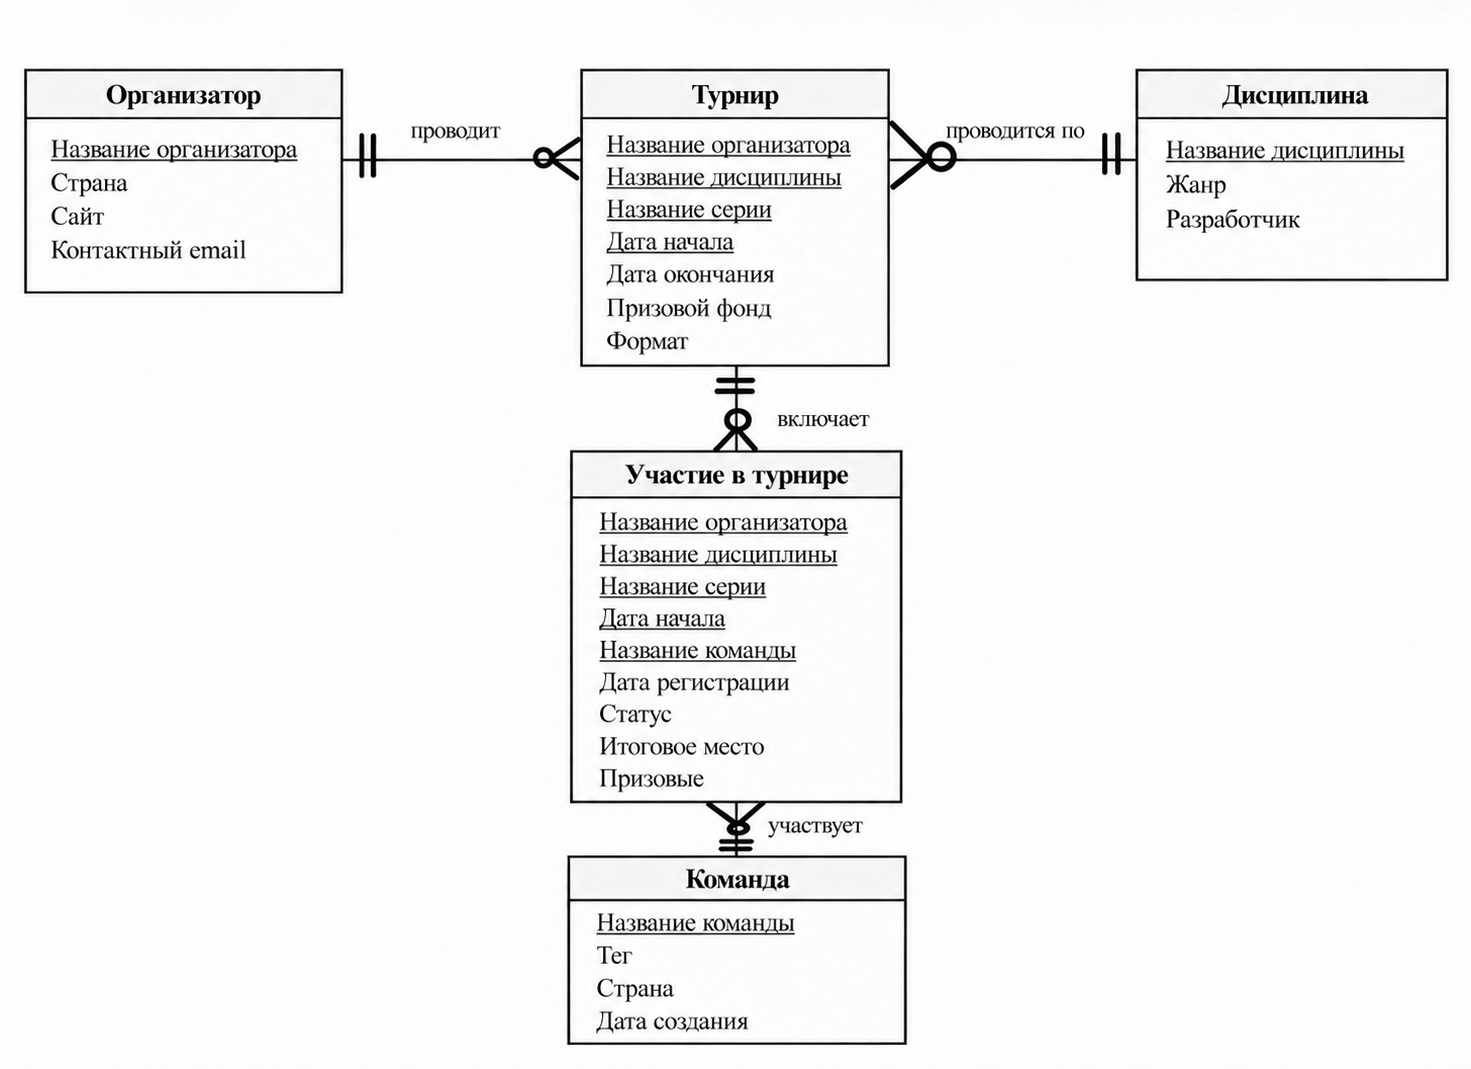
\includegraphics[width=0.93\textwidth]{labdb1.png}
  \caption{Модель <<сущность--связь>> из лабораторной работы № 1}
  \label{fig:er-model}
\end{figure}

\clearpage
Получены пять отношений. Связь турниров и команд реализована через отношение <<Участие в турнире>>. Реляционная модель приведена на рисунке~\ref{fig:rel-model}.

\begin{figure}[H]
  \centering
  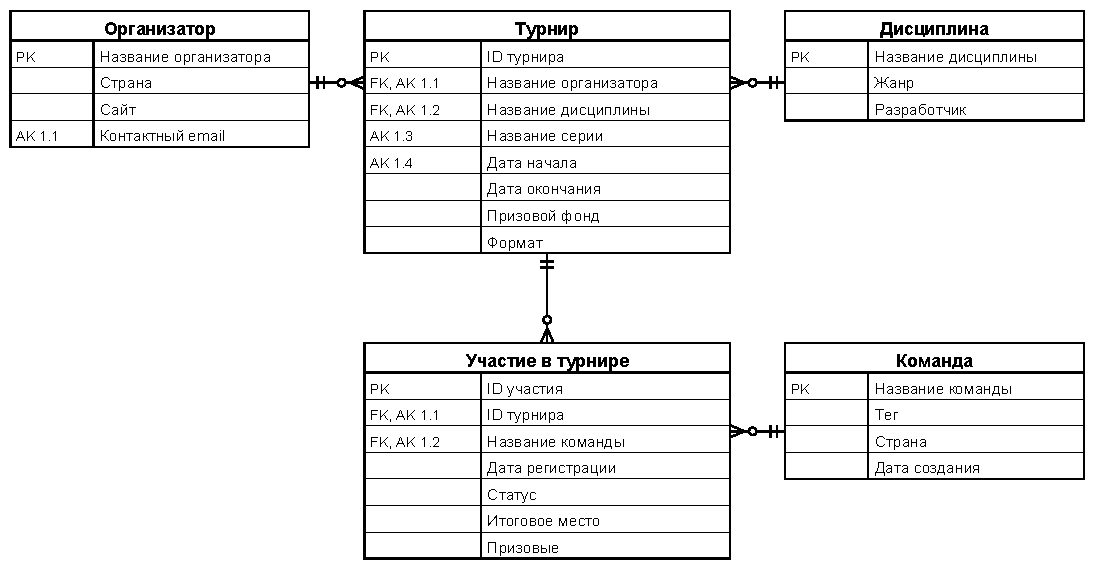
\includegraphics[width=\textwidth]{lab3_schema.pdf}
  \caption{Реляционная модель предметной области}
  \label{fig:rel-model}
\end{figure}

\subsection{Типы данных и ключи}
В таблицах~\ref{tab:org}--\ref{tab:part} приведены атрибуты отношений, типы данных, ключи и допустимость неопределённых значений. Составные идентификаторы турнира и участия сохранены как AK1; уникальна полная комбинация его полей.

\begin{table}[H]
\caption{Отношение <<Организатор>>}
\label{tab:org}
\centering
\fontsize{10.5}{12.6}\selectfont
\setlength{\tabcolsep}{4pt}
\renewcommand{\arraystretch}{1.12}
\begin{tabularx}{\textwidth}{|L{3.5cm}|L{2.3cm}|L{2.0cm}|L{1.9cm}|Y|}
\hline
\textbf{Атрибут} & \textbf{Тип данных} & \textbf{Ключ} & \textbf{NULL} & \textbf{Примечание} \\ \hline
Название организатора & nvarchar(255) & PK & \mbox{NOT NULL} & Уникальное название \\ \hline
Страна & char(2) & - & \mbox{NOT NULL} & Код страны, например RU \\ \hline
Сайт & nvarchar(2048) & - & \mbox{NULL} & Официальный сайт \\ \hline
Контактный email & varchar(254) & AK 1.1 & \mbox{NOT NULL} & Уникальный адрес \\ \hline
\end{tabularx}
\end{table}

\begin{table}[H]
\caption{Отношение <<Дисциплина>>}
\label{tab:disc}
\centering
\fontsize{10.5}{12.6}\selectfont
\setlength{\tabcolsep}{4pt}
\renewcommand{\arraystretch}{1.12}
\begin{tabularx}{\textwidth}{|L{3.5cm}|L{2.3cm}|L{2.0cm}|L{1.9cm}|Y|}
\hline
\textbf{Атрибут} & \textbf{Тип данных} & \textbf{Ключ} & \textbf{NULL} & \textbf{Примечание} \\ \hline
Название дисциплины & nvarchar(255) & PK & \mbox{NOT NULL} & Уникальное название \\ \hline
Жанр & nvarchar(255) & - & \mbox{NOT NULL} & Жанр дисциплины \\ \hline
Разработчик & nvarchar(255) & - & \mbox{NOT NULL} & Разработчик игры \\ \hline
\end{tabularx}
\end{table}

\clearpage
Продолжение описания отношений приведено в таблицах~\ref{tab:tour}--\ref{tab:part}.

\begin{table}[H]
\caption{Отношение <<Турнир>>}
\label{tab:tour}
\centering
\fontsize{10.5}{12.6}\selectfont
\setlength{\tabcolsep}{4pt}
\renewcommand{\arraystretch}{1.12}
\begin{tabularx}{\textwidth}{|L{3.5cm}|L{2.3cm}|L{2.0cm}|L{1.9cm}|Y|}
\hline
\textbf{Атрибут} & \textbf{Тип данных} & \textbf{Ключ} & \textbf{NULL} & \textbf{Примечание} \\ \hline
ID турнира & int & PK & \mbox{NOT NULL} & Суррогатный идентификатор \\ \hline
Название организатора & nvarchar(255) & FK, AK 1.1 & \mbox{NOT NULL} & $\to$  Организатор (Название организатора) \\ \hline
Название дисциплины & nvarchar(255) & FK, AK 1.2 & \mbox{NOT NULL} & $\to$  Дисциплина (Название дисциплины) \\ \hline
Название серии & nvarchar(255) & AK 1.3 & \mbox{NOT NULL} & Часть составного AK1 \\ \hline
Дата начала & date & AK 1.4 & \mbox{NOT NULL} & Часть составного AK1 \\ \hline
Дата окончания & date & - & \mbox{NOT NULL} & Не раньше даты начала \\ \hline
Призовой фонд & decimal(15,2) & - & \mbox{NOT NULL} & Сумма в USD; неотрицательная \\ \hline
Формат & nvarchar(255) & - & \mbox{NOT NULL} & Формат проведения \\ \hline
\end{tabularx}
\end{table}

\begin{table}[H]
\caption{Отношение <<Команда>>}
\label{tab:team}
\centering
\fontsize{10.5}{12.6}\selectfont
\setlength{\tabcolsep}{4pt}
\renewcommand{\arraystretch}{1.12}
\begin{tabularx}{\textwidth}{|L{3.5cm}|L{2.3cm}|L{2.0cm}|L{1.9cm}|Y|}
\hline
\textbf{Атрибут} & \textbf{Тип данных} & \textbf{Ключ} & \textbf{NULL} & \textbf{Примечание} \\ \hline
Название команды & nvarchar(255) & PK & \mbox{NOT NULL} & Уникальное название \\ \hline
Тег & nvarchar(255) & - & \mbox{NOT NULL} & Сокращение названия \\ \hline
Страна & char(2) & - & \mbox{NOT NULL} & Код страны, например RU \\ \hline
Дата создания & date & - & \mbox{NULL} & Может быть неизвестна \\ \hline
\end{tabularx}
\end{table}

\begin{table}[H]
\caption{Отношение <<Участие в турнире>>}
\label{tab:part}
\centering
\fontsize{10.5}{12.6}\selectfont
\setlength{\tabcolsep}{4pt}
\renewcommand{\arraystretch}{1.12}
\begin{tabularx}{\textwidth}{|L{3.5cm}|L{2.3cm}|L{2.0cm}|L{1.9cm}|Y|}
\hline
\textbf{Атрибут} & \textbf{Тип данных} & \textbf{Ключ} & \textbf{NULL} & \textbf{Примечание} \\ \hline
ID участия & int & PK & \mbox{NOT NULL} & Суррогатный идентификатор \\ \hline
ID турнира & int & FK, AK 1.1 & \mbox{NOT NULL} & $\to$  Турнир(ID турнира) \\ \hline
Название команды & nvarchar(255) & FK, AK 1.2 & \mbox{NOT NULL} & $\to$  Команда (Название команды) \\ \hline
Дата регистрации & date & - & \mbox{NOT NULL} & Дата регистрации команды \\ \hline
Статус & nvarchar(255) & - & \mbox{NOT NULL} & Статус участия \\ \hline
Итоговое место & varchar(20) & - & \mbox{NULL} & Например, 1, 2, 3-4 \\ \hline
Призовые & decimal(15,2) & - & \mbox{NULL} & Сумма в USD; неотрицательная \\ \hline
\end{tabularx}
\end{table}

\clearpage
\subsection{Ограничения связей}
Характеристики каждой связи и её внешний ключ приведены в таблице~\ref{tab:relations}.

\begin{table}[H]
\caption{Характеристики связей}
\label{tab:relations}
\centering
\fontsize{10.5}{12.6}\selectfont
\setlength{\tabcolsep}{4pt}
\renewcommand{\arraystretch}{1.12}
\begin{tabularx}{\textwidth}{|L{3.1cm}|L{3.9cm}|L{3.5cm}|Y|}
\hline
\textbf{Родитель --- потомок} & \textbf{Тип связи} & \textbf{Потомков у родителя / родителей у потомка} & \textbf{FK потомка} \\ \hline
Организатор --- Турнир & Неидентифицирующая, 1:N, M--O & 0..N / 1..1 & Название организатора; обязательный \\ \hline
Дисциплина --- Турнир & Неидентифицирующая, 1:N, M--O & 0..N / 1..1 & Название дисциплины; обязательный \\ \hline
Турнир --- Участие в турнире & Неидентифицирующая, 1:N, M--O & 0..N / 1..1 & ID турнира; обязательный \\ \hline
Команда --- Участие в турнире & Неидентифицирующая, 1:N, M--O & 0..N / 1..1 & Название команды; обязательный \\ \hline
\end{tabularx}
\end{table}

В таблицах~\ref{tab:org-tour}--\ref{tab:disc-tour} приведены правила действий для связей организатора и дисциплины с турниром.

\begin{table}[H]
\caption{Правила для связи <<Организатор --- Турнир>>}
\label{tab:org-tour}
\centering
\fontsize{11}{13.2}\selectfont
\setlength{\tabcolsep}{5pt}
\renewcommand{\arraystretch}{1.12}
\begin{tabularx}{\textwidth}{|L{2.5cm}|Y|Y|}
\hline
\textbf{Операция} & \textbf{Организатор (родитель)} & \textbf{Турнир (потомок)} \\ \hline
Вставка & Разрешено. & Разрешено, если указан существующий организатор и AK1 уникален. \\ \hline
Изменение PK / FK & Разрешено, если новое название уникально; ссылки обновляются согласованно. & Разрешено, если новый организатор существует и AK1 уникален. \\ \hline
Удаление & Разрешено, если нет связанных турниров. & Запрещено. \\ \hline
\end{tabularx}
\end{table}

\begin{table}[H]
\caption{Правила для связи <<Дисциплина --- Турнир>>}
\label{tab:disc-tour}
\centering
\fontsize{11}{13.2}\selectfont
\setlength{\tabcolsep}{5pt}
\renewcommand{\arraystretch}{1.12}
\begin{tabularx}{\textwidth}{|L{2.5cm}|Y|Y|}
\hline
\textbf{Операция} & \textbf{Дисциплина (родитель)} & \textbf{Турнир (потомок)} \\ \hline
Вставка & Разрешено. & Разрешено, если указана существующая дисциплина и AK1 уникален. \\ \hline
Изменение PK / FK & Разрешено, если новое название уникально; ссылки обновляются согласованно. & Разрешено, если новая дисциплина существует и AK1 уникален. \\ \hline
Удаление & Разрешено, если нет связанных турниров. & Запрещено. \\ \hline
\end{tabularx}
\end{table}

\clearpage
В таблицах~\ref{tab:tour-part}--\ref{tab:team-part} приведены правила действий для связей турнира и команды с участием. Запись участия относится к исходным турниру и команде; переименование команды сохраняет эту связь.

\begin{table}[H]
\caption{Правила для связи <<Турнир --- Участие в турнире>>}
\label{tab:tour-part}
\centering
\fontsize{11}{13.2}\selectfont
\setlength{\tabcolsep}{5pt}
\renewcommand{\arraystretch}{1.12}
\begin{tabularx}{\textwidth}{|L{2.5cm}|Y|Y|}
\hline
\textbf{Операция} & \textbf{Турнир (родитель)} & \textbf{Участие в турнире (потомок)} \\ \hline
Вставка & Разрешено. & Разрешено, если указан существующий турнир и AK1 уникален. \\ \hline
Изменение PK / FK & Запрещено. & Запрещено. \\ \hline
Удаление & Запрещено. & Разрешено. \\ \hline
\end{tabularx}
\end{table}

\begin{table}[H]
\caption{Правила для связи <<Команда --- Участие в турнире>>}
\label{tab:team-part}
\centering
\fontsize{11}{13.2}\selectfont
\setlength{\tabcolsep}{5pt}
\renewcommand{\arraystretch}{1.12}
\begin{tabularx}{\textwidth}{|L{2.5cm}|Y|Y|}
\hline
\textbf{Операция} & \textbf{Команда (родитель)} & \textbf{Участие в турнире (потомок)} \\ \hline
Вставка & Разрешено. & Разрешено, если указана существующая команда и AK1 уникален. \\ \hline
Изменение PK / FK & Разрешено, если новое название уникально; ссылки обновляются согласованно. & Разрешено только при переименовании той же команды. \\ \hline
Удаление & Разрешено, если нет связанных участий. & Разрешено. \\ \hline
\end{tabularx}
\end{table}

\section{Вывод}
Построена реляционная модель из пяти таблиц. Определены типы данных, ключи и правила действий для каждой связи.

\end{document}
